\documentclass{beamer}

\usetheme{Copenhagen}

\usepackage{listings}
\usepackage{graphicx}
\usepackage{caption}
\usepackage{subcaption}

\title{Using Processing with Java}

\subtitle{Introduction}

\author{Eduardo Sousa \\eduardosousa@ua.pt}

\institute[University of Aveiro]{University of Aveiro}

\date{2016}

\subject{Computer Science}

\graphicspath{{images/}}

\begin{document}

\defverbatim[colored]\lstCodeStruct{
	\begin{lstlisting}[language=Java,basicstyle=\ttfamily,tabsize=4]
public class Teste extends PApplet {
	public static void main(String[] args) {
		PApplet.main(Teste.class.getName());
	}

	public void settings() {...}

	public void setup() {...}

	public void draw() {...}
}
	\end{lstlisting}
}

\defverbatim[colored]\lstCanvasFunctions{
	\begin{lstlisting}[language=Java,basicstyle=\ttfamily,tabsize=4]
	// Can only be used in settings()
	size(width, heigth);

	// Cannot be used in settings()
	// 0 <= grey, r, g, b <= 255
	background(grey);
	background(r, g, b);
	\end{lstlisting}
}

\defverbatim[colored]\lstStroke{
	\begin{lstlisting}[language=Java,basicstyle=\ttfamily,tabsize=4]
	// No border
	noStroke();

	// Size of line - default = 1
	strokeWeight(weight);

	// alpha == transparency
	// 0 <= grey, r, g, b, alpha <= 255
	stroke(grey);
	stroke(r, g, b);
	stroke(r, g, b, alpha);
	\end{lstlisting}
}

\defverbatim[colored]\lstFill{
	\begin{lstlisting}[language=Java,basicstyle=\ttfamily,tabsize=4]
	// No fill
	noFill();

	// alpha == transparency
	// 0 <= grey, r, g, b, alpha <= 255
	fill(grey);
	fill(r, g, b);
	fill(r, g, b, alpha);
	\end{lstlisting}
}

\defverbatim[colored]\lstImages{
	\begin{lstlisting}[language=Java,basicstyle=\ttfamily,tabsize=4]
	// Declaring the image object
	PImage img;

	// Loading the image
	img = loadImage("img.jpg");

	// Showing the image
	image(img, x, y);

	// Resizing and showing the image
	iamge(img, x, y, width, heigth);
	\end{lstlisting}
}

\defverbatim[colored]\lstSounds{
	\begin{lstlisting}[language=Java,basicstyle=\ttfamily,tabsize=4]
	import processing.sound.*;
	
	// Declaring the sound file
	SoundFile sound;

	// Loading the sound file
	sound = new SoundFile(this, "song.mp3");

	// Playing the sound
	sound.play();

	// Playing the sound file in a loop
	sound.loop();
	\end{lstlisting}
}

\defverbatim[colored]\lstMouse{
	\begin{lstlisting}[language=Java,basicstyle=\ttfamily,tabsize=4]
	public void mousePressed() {...}
	public void mouseReleased() {...}
	public void mouseClicked() {...}
	public void mouseDragged() {...}
	public void mouseMoved() {...}
	public void mouseWheel() {...}
	\end{lstlisting}
}

\defverbatim[colored]\lstKeyboard{
	\begin{lstlisting}[language=Java,basicstyle=\ttfamily,tabsize=4]
	public void keyPressed() {...}

	public void keyReleased() {...}
	\end{lstlisting}
}

\defverbatim[colored]\lstKeyboardExample{
	\begin{lstlisting}[language=Java,basicstyle=\ttfamily,tabsize=4]
	public void keyPressed() {
		if(key == 'p' || key == 'P') {
			pauseTheGame();
		} else if(key == CODED) {
			if(keyCode == UP) {
				goUp();
			} else if(keyCode == DOWN) {
				goDown();
			}
		}
	}
	\end{lstlisting}
}

\begin{frame}
  \titlepage
\end{frame}

\section{Introduction}

\subsection{Setup}

\begin{frame}{Code Structure}
\lstCodeStruct
\end{frame}

\subsection{Canvas}

\begin{frame}{What is the canvas?}
The canvas is the window where all the objects will be drawn.

\begin{figure}[H]
\centerline{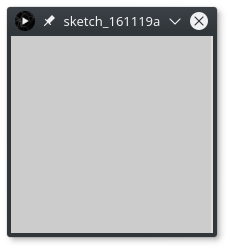
\includegraphics[scale=0.5]{canvas.png}}
\caption{Canvas}
\end{figure}
\end{frame}

\begin{frame}{Canvas coordinate system}
This is the canvas coordinate system.\\
Objects will only be drawn if they are inside the canvas,
 e.g. \textit{rect(1, 2, 2, 2)}.

\begin{figure}[H]
\centerline{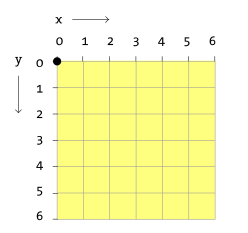
\includegraphics[scale=0.5]{canvas_coordinate_system.png}}
\caption{Canvas coordinate system}
\end{figure}
\end{frame}

\begin{frame}{Canvas functions}
Functions needed to alter the canvas:

\lstCanvasFunctions
\end{frame}

\subsection{Drawing Loop}

\begin{frame}{Drawing Loop}
In Processing, the drawing loop is based in frames.
Each time a new frame is going to be presented in the display,
Processing will call the function \textbf{draw()}.\\ 
The default frame rate is 60 frames per second, so in this case, 
every second the function \textbf{draw()} will be called 60 times.
\end{frame}

\begin{frame}{Stoping drawing loop}
To stop the the drawing loop, use \textbf{noLoop()}.\\
This will freeze the moving objects in the canvas.\\

Can be useful for pausing a game.
\end{frame}

\begin{frame}{Drawing a new frame}
If the drawing loop is stopped, you can use \textbf{redraw()} to 
render a new frame, without restarting the drawing loop.\\

Can be useful to draw a menu when the game is paused.
\end{frame}

\begin{frame}{Resuming drawing loop}
If the drawing loop is stopped, you can use \textbf{loop()} to
restart the drawing loop.\\

Can be useful when you are resuming the game after a pause.
\end{frame}

\section{Drawing Functions}

\begin{frame}{Drawing instruction order}
For every object you are going to draw, there is an order to call
the drawing functions.\\

\begin{enumerate}
\item{Stroke/Fill}
\item{Mode}
\item{Object}
\end{enumerate}
\end{frame}

\subsection{Stroke}

\begin{frame}{Stroke}
Stroke is the border line of the objects. It can be defined using the following functions.\\

\lstStroke
\end{frame}

\subsection{Fill}

\begin{frame}{Fill}
Fill is the color of the object. It can be defined using the following functions.\\

\lstFill
\end{frame}

\subsection{Point}

\begin{frame}{Point}
To draw a point, use the function \textbf{point(x, y)}.

\begin{figure}[H]
\centerline{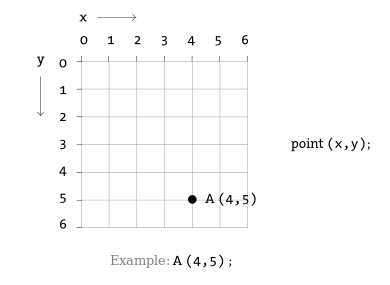
\includegraphics[scale=0.5]{point.png}}
\caption{Point}
\end{figure}
\end{frame}

\subsection{Line}

\begin{frame}{Line}
To draw a line, use the function \textbf{line(x1, y1, x2, y2)}.

\begin{figure}[H]
\centerline{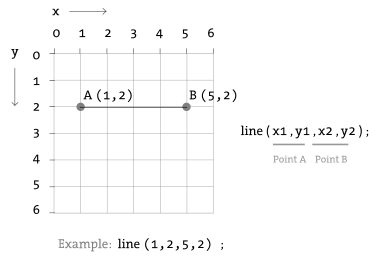
\includegraphics[scale=0.5]{line.png}}
\caption{Line}
\end{figure}
\end{frame}

\subsection{Rect}

\begin{frame}{Rectangle - RectMode = CORNER}
To draw a rectangle, use the function \textbf{rect(x, y, width, heigth)}.\\
The default mode for drawing a rectangle is the CORNER, where the upper
left corner will be used as the reference point.\\

\begin{figure}[H]
\centerline{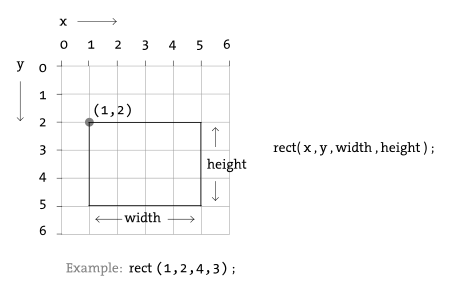
\includegraphics[scale=0.5]{rectangle_corner_mode.png}}
\caption{Rectangle - CORNER mode}
\end{figure}
\end{frame}

\begin{frame}{Rectangle - RectMode = CENTER}
To draw a rectangle, where the reference point is the center, use the
functions as defined below:\\

\begin{figure}[H]
\centerline{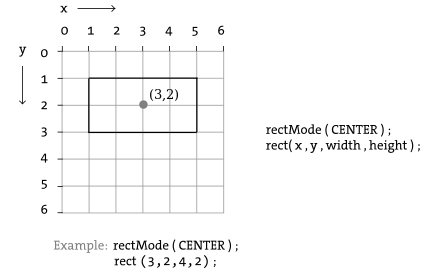
\includegraphics[scale=0.5]{rectangle_center_mode.png}}
\caption{Rectangle - CENTER mode}
\end{figure}
\end{frame}

\begin{frame}{Rectangle - RectMode = CORNERS}
To draw a rectangle, where the reference points are upper left corner
and lower right corner, use the function as defined below:\\

\begin{figure}[H]
\centerline{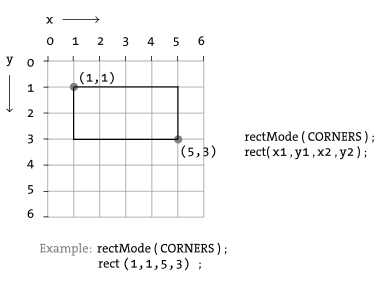
\includegraphics[scale=0.5]{rectangle_corners_mode.png}}
\caption{Rectangle - CORNERS mode}
\end{figure}
\end{frame}

\subsection{Ellipse}

\begin{frame}{Ellipse - EllipseMode = CENTER}
To draw an ellipse, use the function \textbf{ellipse(x, y, width, heigth)}.\\
The default mode for drawing an ellipse is the CENTER, where the center will
be used as the reference point.\\

\begin{figure}[H]
\centerline{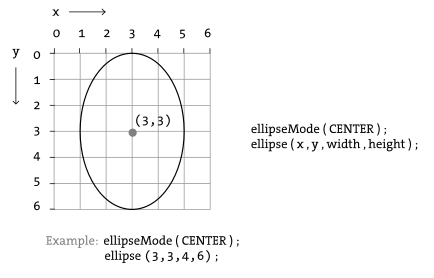
\includegraphics[scale=0.5]{ellipse_center_mode.png}}
\caption{Ellipse - CENTER mode}
\end{figure}
\end{frame}

\begin{frame}{Ellipse - EllipseMode = CORNER}
To draw an ellipse, where the reference point is the upper left corner, use
the functions as defined below:\\

\begin{figure}[H]
\centerline{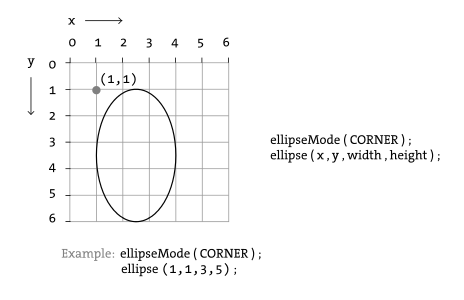
\includegraphics[scale=0.5]{ellipse_corner_mode.png}}
\caption{Ellipse - CORNER mode}
\end{figure}
\end{frame}

\begin{frame}{Ellipse - EllipseMode = CORNERS}
To draw an ellipse, where the reference points are the upper left coner and 
the lower right corner, use the functions as defined below:\\

\begin{figure}[H]
\centerline{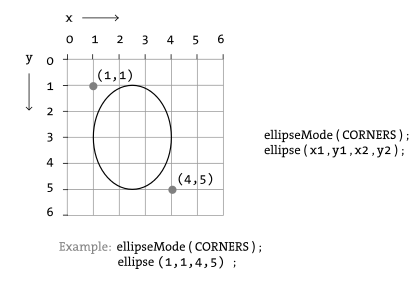
\includegraphics[scale=0.5]{ellipse_corners_mode.png}}
\caption{Ellipse - CORNERS mode}
\end{figure}
\end{frame}

\subsection{Images}

\begin{frame}{Using images}
To use images, use the following code:\\

\lstImages

It supports the following formats: GIF, JPG, TGA, PNG.
\end{frame}

\subsection{Sound}

\begin{frame}{Using sound}
To use sounds, use the following code:\\

\lstSounds

It supports the following formats: WAV, AIF/AIFF, MP3.
\end{frame}

\section{Interaction Functions}

\subsection{Mouse Interactions}

\begin{frame}{Using the mouse variables}
In Processing, the mouse can only be used when the pointer
is over the canvas.\\
There are some variables that are useful when using the mouse:

\begin{itemize}
\item{\textbf{mouseX} - current X coordinate of the mouse pointer}
\item{\textbf{mouseY} - current Y coordinate of the mouse pointer}
\item{\textbf{pmouseX} - previous X coordinate of the mouse pointer}
\item{\textbf{pmouseY} - previous Y coordinate of the mouse pointer}
\item{\textbf{mousePressed} - true if the mouse is currently being pressed}
\item{\textbf{mouseButton} - indicates which button of the mouse is being pressed (LEFT or RIGHT)}
\end{itemize}
\end{frame}

\begin{frame}{Using mouse functions}
If one of the mouse actions happens, one or more of the following functions will be called:\\

\lstMouse

\textbf{Note: } you don't need to implement all these functions.\\
Implement the ones that are needed.
\end{frame}

\subsection{Keyboard Interactions}

\begin{frame}{Using keyboard variables}
There are few variables that hold values when a key is pressed.\\
These are the variables:\\

\begin{itemize}
\item{\textbf{keyPressed} - true if there is a key being pressed}
\item{\textbf{key} - key value if keyPressed == true}
\item{\textbf{keyCode} - if key == CODED, keyCode will hold the code}
\end{itemize}
\end{frame}

\begin{frame}{Coded Keys}
If the key is not specified in the ASCII code, you will have to use 
the \textbf{keyCode} variable to check what is the value.\\
Here you the most used keys that are coded:\\

\begin{itemize}
\item{UP}
\item{DOWN}
\item{LEFT}
\item{RIGHT}
\item{ALT}
\item{SHIFT}
\item{CONTROL}
\end{itemize}
\end{frame}

\begin{frame}{Using keyboard functions}
If one of the keyboard actions happens, one or more of the following functions will be called:\\

\lstKeyboard

\textbf{Note: } you don't need to implement all these functions.\\
Implement the ones that are needed.
\end{frame}

\begin{frame}{Coded keys - Example}
Here is an example of the use of coded keys:\\

\lstKeyboardExample
\end{frame}

\section{References}

\begin{frame}{References}
If you need more specific information, check these links:\\

\begin{itemize}
\item{\url{https://processing.org/reference/}}
\item{\url{https://processing.org/reference/libraries/}}
\item{\url{https://processing.org/tutorials/}}
\item{\url{https://processing.org/examples/}}
\end{itemize}
\end{frame}

\end{document}
